% ------------------------------------------------------------------------------
% AppSensor Overview
% For OWASP AppSec USA November 20th, 2013
% by Dennis Groves
% ------------------------------------------------------------------------------

\documentclass[leqno]{beamer}

\usetheme{OWASP}

% packages
\usepackage{amssymb,amsmath} % math layout
\usepackage{color} % if you want colored text in your document
\usepackage[export]{adjustbox} % Adjust figure placement on page
\usepackage{graphicx}
\usepackage[orientation=landscape,size=custom,width=14.4,height=9,scale=0.5]{beamerposter} % Resize slides fit macbook air display
\usepackage[pdftex]{thumbpdf} % produce slide thumbnails for pdf readers
\usepackage{textcomp}
\usepackage{textpos}
\usepackage{tikz}
\usepackage{url} % help you typeset URLs
\usepackage{xltxtra} % Extra customizations for XeLaTeX;
% xltxtra automatically loads fontspec and xunicode, both of which you need
    \defaultfontfeatures{Mapping=tex-text,Scale=MatchLowercase}
    \setsansfont[Scale=MatchLowercase,Mapping=tex-text]{Armata-Regular.otf}
    \setbeamerfont{frametitle}{size=\LARGE,series=\bfseries}
    \usefonttheme{professionalfonts}
    
\setbeamertemplate{navigation symbols}{} % remove navigation at bottom of slides

% Title Content
\title{OWASP AppSensor\\ The Future of Application Security} 
\author[Dennis Groves]{Dennis Groves, MSc\\ dennis.groves@owasp.org} 

\graphicspath{{images/}} % default place to search for presentation images

%%%%%%%%%%%%%%%%%%%%%%%%%%%%%%%%%%%%%%%%%%%%%%%%%%%%%%%%%%%%%%%%%%%%%%%%%%%%%
%% Begin Slides
%%%%%%%%%%%%%%%%%%%%%%%%%%%%%%%%%%%%%%%%%%%%%%%%%%%%%%%%%%%%%%%%%%%%%%%%%%%%%
\begin{document}{

%
% SLIDE  ----------------------------------------------------------
%

{
\begin{frame}[plain]
   \titlepage
\end{frame}
}

%% ABOUT ME %%%%%%%%%%%%%%%%%%%%%%%%%%%%%%%%%%%%%%%%%%%%%%%%%%%%%%%%

%
% SLIDE  ----------------------------------------------------------
%

{
\frame{\frametitle{About Me}
	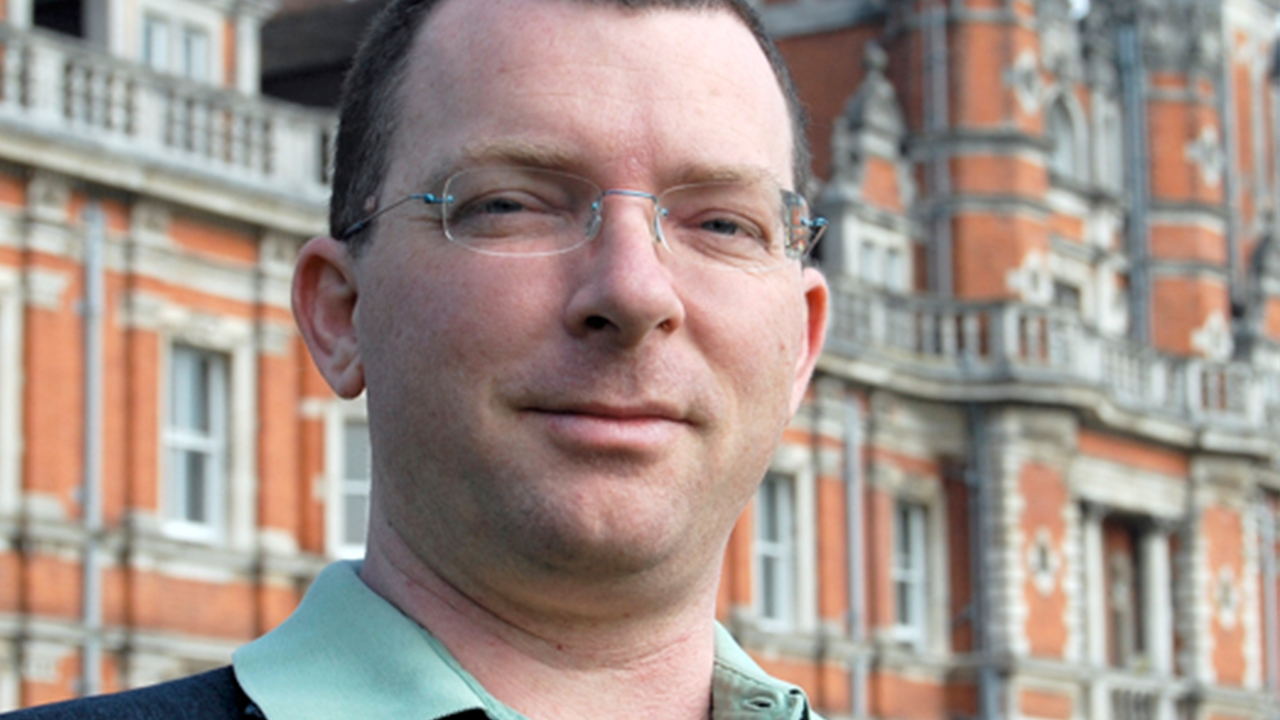
\includegraphics[width=.9\textwidth, center]{dennis}
}

%% PISTOL DUELING %%%%%%%%%%%%%%%%%%%%%%%%%%%%%%%%%%%%%%%%%%%%%%%%%%%%%%%%

%% I would like to start the philosophy discussion with a thought exercise. This is the thought exercise. Tomorrow we have a pistol duel.  If we loose we will be shot and likely die, if we win our opponent takes the bullet instead and suffers a similar fate as we should we loose. Lets agree to the following process which matches our information security management practices. We will do a risk analysis, then reduce the risks identified and then we will go have our duel. So the question is what do we do to ensure our survival? Lets begin our risk analysis now. We need far more information in order to survive. 

%
% SLIDE  ----------------------------------------------------------
%
\frame{\frametitle{A Thought Experiment}
    
\includegraphics[width=1\textwidth, center]{BeakerBunsen}
}

%% To begin with we seem to it would be really important to know what the rules of our pistol duel are. Incidentally, there are two types of pistol duels. There are Victorian and Western Pistol duels.  And depending on which we are participating in greatly changes both our risks and the strategies we require to survive.

%
% SLIDE  ----------------------------------------------------------
%
\frame{\frametitle{OPSEC}
    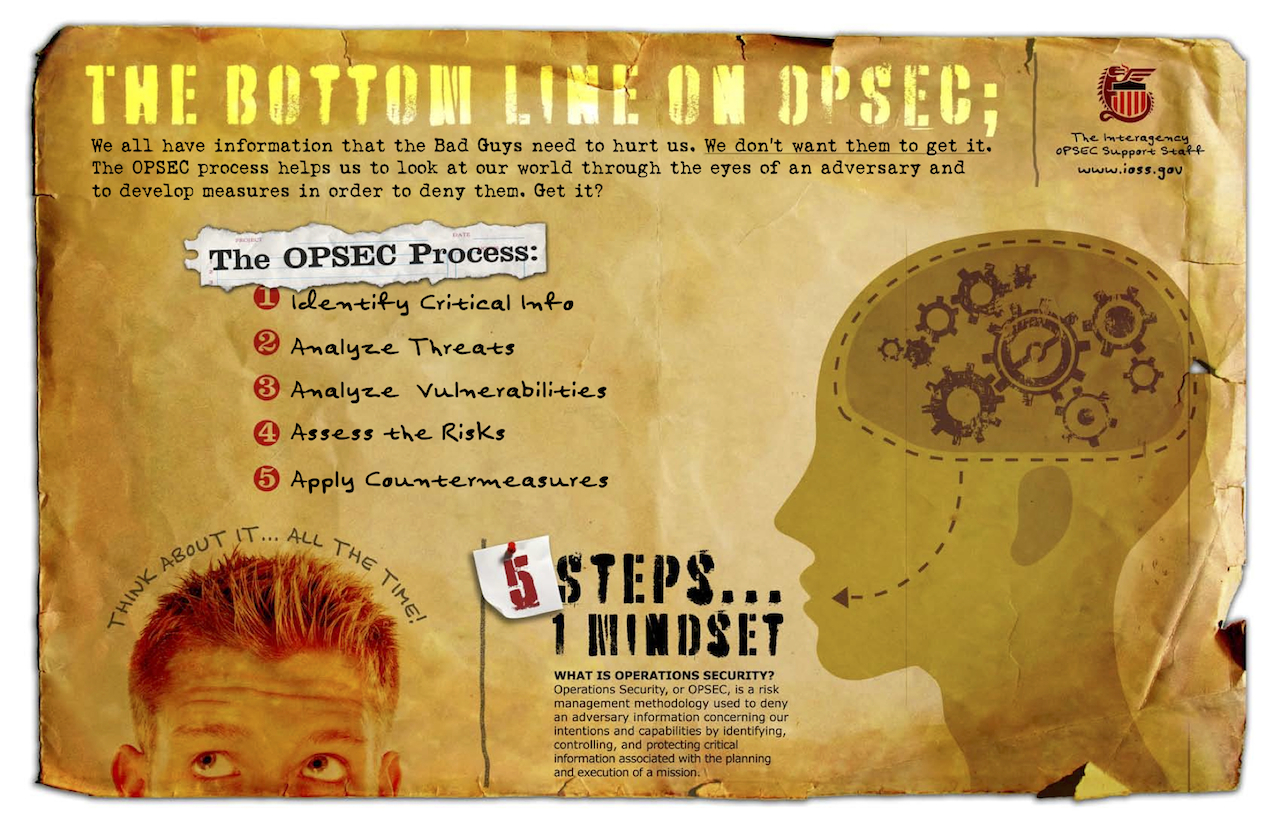
\includegraphics[width=.9\textwidth, center]{OPSEC}
}

%
% SLIDE  ----------------------------------------------------------
%
\frame{\frametitle{1: Identify Critical Info}
    
\includegraphics[width=1\textwidth, center]{rodin_thinker}
}

%% Identity
% Self-awareness
%  - without it, all threats apparently emanate from oneself
%  - you are your own worst enemy
%
% Differentiation between self and others (singular)
%  - me and you
%
% Differentiation between trusted and untrusted groups (many)
%  - us vs them
%  - trust
%  - boundaries
%
% Hygene Hypothesis
%  - if you succeed in destroying them, you will destroy yourself.
%  - "security does'nt exist & entropy will get you in the end."

%
% SLIDE  ----------------------------------------------------------
%
\frame{\frametitle{Know Yourself}
	\begin{columns}
		\begin{column}{.45\textwidth}
			 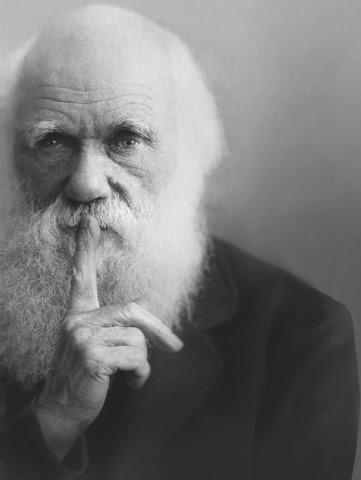
\includegraphics[width=1\textwidth]{darwin.png}
        \end{column}
	\begin{column}{.45\textwidth}
		\begin{quote}
			"It is not the strongest of the species that survives, nor the most intelligent that survives. It is the one that is the most adaptable to change."
		\end{quote}		
	\end{column}
\end{columns}
}

%% In a Victorian pistol duel, opponents stand back to back, take ten steps away from each other, turn and fire. The fairness of this kind of duel depends on neither party turning at step 9 or earlier. So it is a game of trust, that depends on neither party cheating. However, cheating means we are not killed. And since our goal is to survive and our pistol duel is a Victorian duel; then we have our first risk reduction strategy! We simply turn after step one and shoot our opponent! 

%
% SLIDE  ----------------------------------------------------------
%
\frame{\frametitle{Vitorian Duel}
    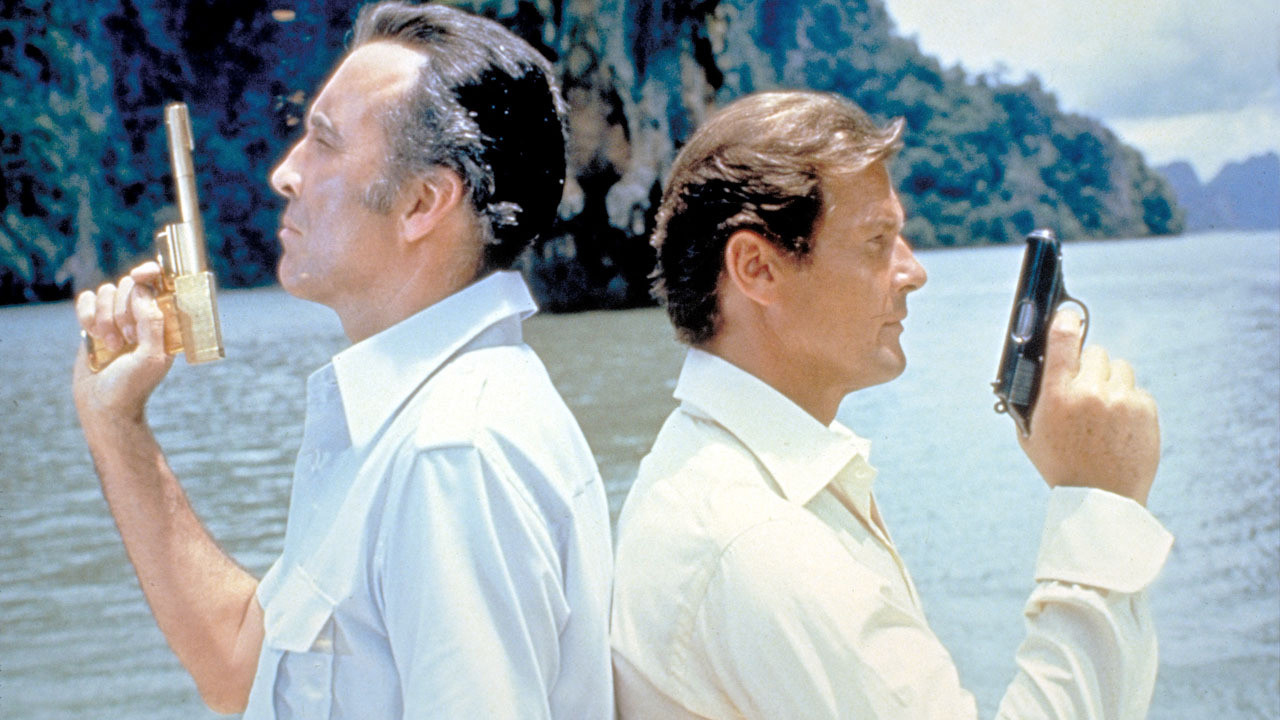
\includegraphics[width=.9\textwidth, center]{victorian}
}

%% Increasing speed, or being faster is a key security metric. In fact it is the entire basis for time based security. Time based security states that our protection time must be greater than or equal to detection time plus response time. A great example of this principle in action was the final scene of the Matrix where Neo can dodge the bullets. He is able to detect and react before the bullets reach him; this causes him to be invincible for all practical purposes. We all know what the longer it takes a vendor to fix our bugs the greater risk we are at, as attackers are able to attack us until we can patch. Similarly, the longer it takes for us to fix our own bugs the more vulnerable we are. This metric can be applied in many circumstances, and I encourage you to try and apply it to things in your environment and to start measuring security from this perspective. 

%
% SLIDE  ----------------------------------------------------------
%
\frame{\frametitle{Use Time Based Security Metrics}
Use Time Based Security Metrics
\begin{theorem}
Protection time must be greater than or equal to detection time plus reaction time.
\end{theorem}
\begin{equation}
	P_{t}\geq D_{t} + R_{t}
\end{equation}
}

%% Now the other kind of duel we maybe having is a western duel. A western duels are the ones in all the westerns where the opponents meet at high noon. We no longer have to trust our opponent, instead we have place and time that decides when the duel begins. Punctuality is important otherwise someone you love will be killed in your place. Opponents face one another from twenty paces and draw pistols from holsters. It is difficult to cheat at the western duel, but you should try anyway. 

%
% SLIDE  ----------------------------------------------------------
%
\frame{\frametitle{Wester Duel}
    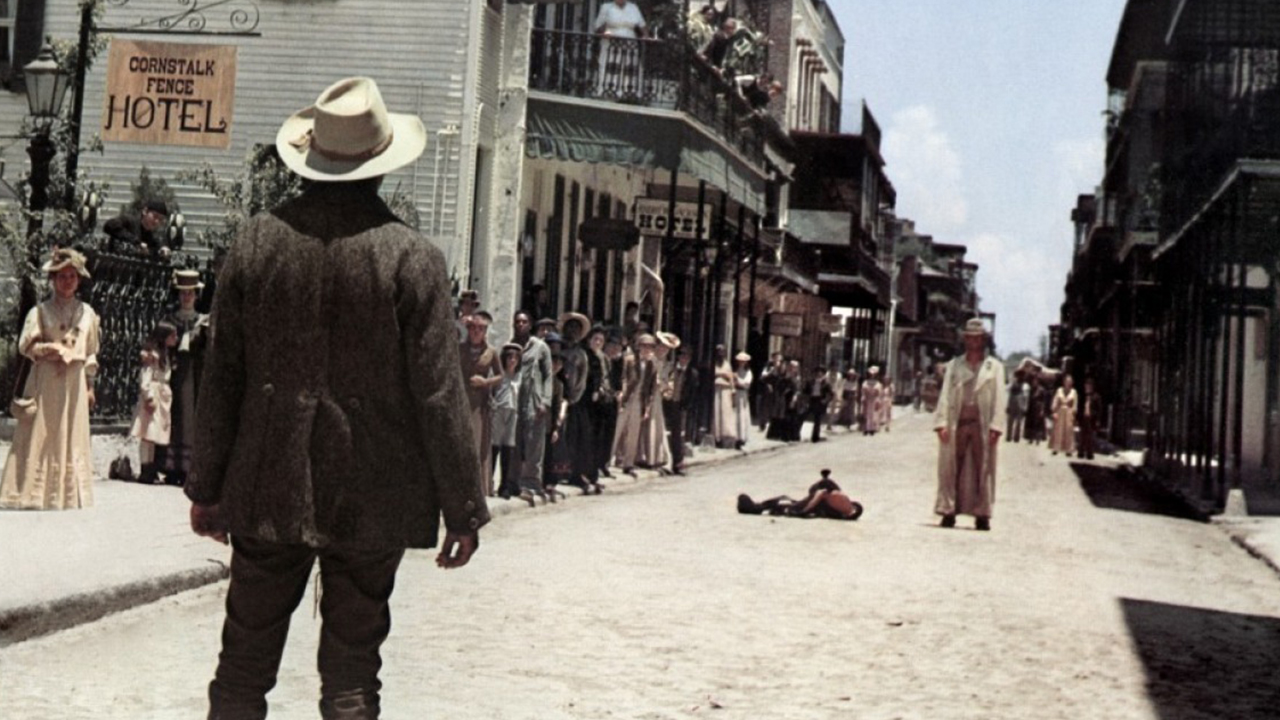
\includegraphics[width=.9\textwidth, center]{western}
}

%% Additionally, I think it is likely a good idea to know whom our opponent is. I personally believe that it is essential otherwise you have no ability to understand the threat you face and mitigate risks accordingly. For example many of us, if we were put in a situation where the opponent were one of our loved ones or immediate family, are very likely to loose on purpose. For the purpose of this exercise however our opponent will be my next door neighbor - a 6 foot 4 inch, 63 year old man. Because of this disadvantage we will face off in a Western duel to keep things fair.


%% I can imagine that most of you right now will be feeling a bit relieved to know that we are facing an old man, and one who has a fairly large surface area to aim for. In application security we very rarely consider who our opponent is, what they are motivated by and how man resources they have at their disposal to attack us. But it is critical. To further emphasize this point I will tell you a bit more about my 63 year old neighbor. His name is Johnny Brusco, and he was the fastest quick draw in the United States until 1974 when he retired from quick draw competition. Suddenly, with a single piece of information our assessment of the risk went from a risk of ‘mostly harmless’ to ‘we are seriously, very dead.’

%
% SLIDE  ----------------------------------------------------------
%
\frame{\frametitle{Know your Opponent}
\begin{columns}[c]
\column{2in}
    \textbf{Pistol Duel}
    \begin{itemize}
        \item{Novice Shooter}
        \item{Weekend Shooter}
        \item{Professional Shooter}
        \item{Quick Draw Champion}
    \end{itemize}
\column{2in}
    \textbf{Application}
    \begin{itemize}
        \item{Script Kiddies}
        \item{Hacktivists}
        \item{Criminals}
        \item{Disgruntled Employee}
        \item{Corporate Spy}
        \item{Cyber Warrior}
    \end{itemize}
\end{columns}
}

%% This scenario is not unlike the one we face with our web applications every day. Attackers significantly out number defenders. Additionally, attackers do not have tight budgets, deadlines and last minute changes to requirements to manage. Attackers only have to find a single vulnerability, defenders have to find and fix them all; something we know can not be done so we rank them in order of importance by perceived risk. Indeed all is not hopeless, industry best practices tell us risk treatment is the ‘best practice’ today. And we can use the same principles here in our duel where we are seriously out gunned by our opponent. 

%
% SLIDE  ----------------------------------------------------------
%
\frame{\frametitle{Out Gunned}
    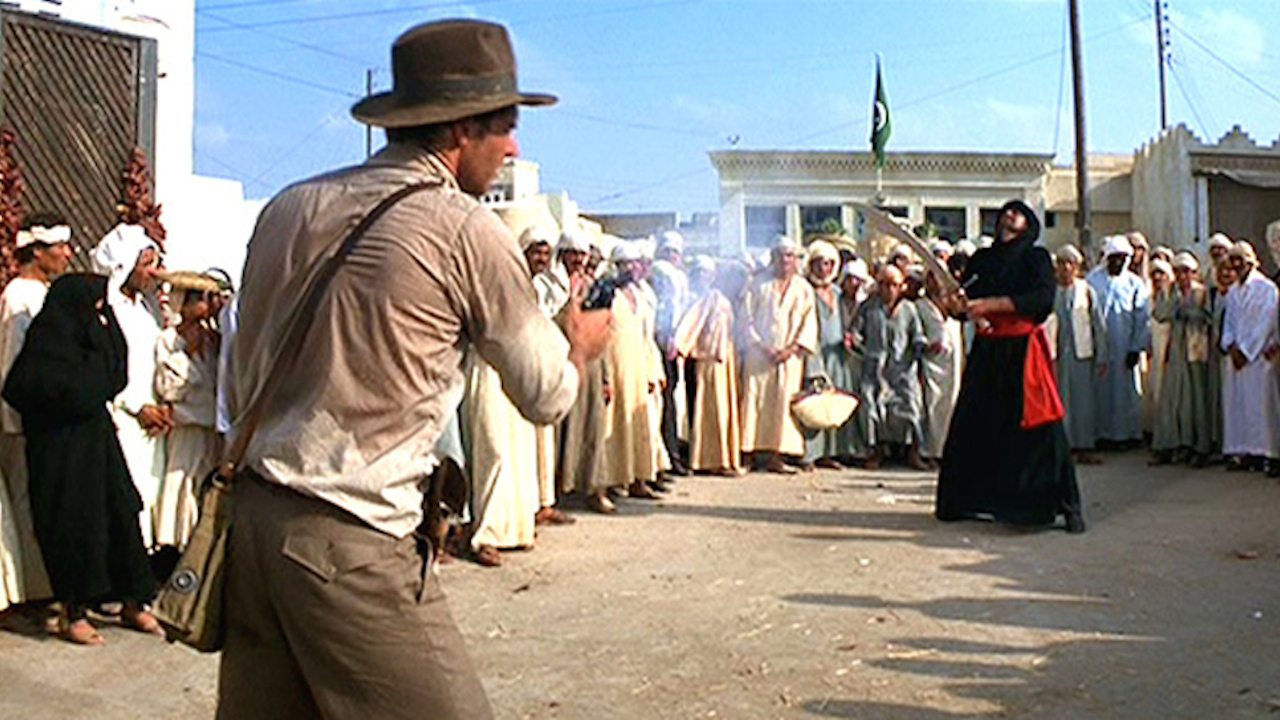
\includegraphics[width=.9\textwidth, center]{indy}
}

%% Risk can be defined simply as the probability of the vulnerability times the threat.  And the two most widely used strategies for managing risk are to reduce the probability of a threat and/or reduce the probability of a vulnerability. To reduce the probability of a threat we reduce the attack surface. This is a fancy way of saying we patch the vulnerabilities that are identified so there are ‘less places for attackers to attack.’ The other thing we do is to hire penetration testers; and to do internal testing of our own security. This is how we identify vulnerabilities. By finding our vulnerabilities before the bad guys we can fix them before they are exploited. 

%
% SLIDE  ----------------------------------------------------------
%
\frame{\frametitle{2: Analyze Threats}
\begin{columns}[c]
\column{2in}
    \textbf{Pistol Duel}
    \begin{itemize}
        \item{Handgun Skills}
        \item{Nervousness}
        \item{Psychological Readiness}
    \end{itemize}
\column{2in}
    \textbf{Application}
    \begin{itemize}
        \item{Spoofing}
        \item{Tampering}
        \item{Repudiation}
        \item{Information Disclosure}
        \item{Denial of Service}
        \item{Elevation of Privilege}
    \end{itemize}
\end{columns}
}


%
% SLIDE  ----------------------------------------------------------
%
\frame{\frametitle{3: Analyze Vulnerabilities}
\begin{columns}[c]
\column{2in}
    \textbf{Pistol Duel}
    \begin{itemize}
        \item{Jam}
        \item{Misfire}
        \item{Backfire}
    \end{itemize}
\column{2in}
    \textbf{The OWASP Top-10}
    \begin{itemize}
        \item{A1 Injection}
        \item{A3 Cross-Site Scripting}
        \item{A5 Security Misconfiguration}
        \item{A7 Missing Access Control}
    \end{itemize}
\end{columns}
}


%
% SLIDE  ----------------------------------------------------------
%
\frame{\frametitle{4: Analyze Risks}

The probable frequency and probable magnitude of future loss

\begin{align}
	\text{Risk = }& \text{P(Impact)}\\
	\text{Risk = }& \text{P(Impact * Vulnerability)}\\
	\text{Risk = }& \text{Impact * Vulnerability * Threat}\\
	\text{Risk = }& \text{P(Impact * Vulnerability * Threat)}\\
	\text{Risk = }& \cfrac{\text{Impact * Vulnerability * Threat}}{\text{Countermeasures}}\\
	\text{Risk = }& \text{Impact * }\cfrac{\text{P(Threat) * P(Vulnerability)}}{\text{Countermeasures}}
\end{align}
}

%
% SLIDE  ----------------------------------------------------------
%
\frame{\frametitle{5: Apply Countermeasures}
\begin{itemize}
	\item Tolerate: Do nothing.
	\item Transfer: Outsource the risk.
	\item Terminate: Eliminate the asset.
	\item Treat: Reduce the risk.
\end{itemize}
}

%% We can apply the same to our gunfight tomorrow. We can reduce our attack surface by not turning so our shoulders are ‘square’ with our opponent which would expose our entire torso to bullets. But rather we can stand perpendicular to our opponent minimizing the surface area of our bodies subject to bullets. We can also reduce our vulnerabilities by hiring a gunslinger to teach us the art of gunslinging and practice. This is like penetration testing, the gunslinger will identify what we are doing wrong and help us to eliminate the bad habits thus reducing our vulnerabilities or bad habits that are likely to get us shot. 

%
% SLIDE  ----------------------------------------------------------
%
\frame{\frametitle{Risk Reduction Methods}
Reducing the risk (treatment) is the most common strategy used today.
\begin{itemize}
	\item Reduce the probability of a threat.
	\item Reduce the probability of a vulnerability.
\end{itemize}
}

%
% SLIDE  ----------------------------------------------------------
%
\frame{\frametitle{Reduce Attack Surface}
\begin{columns}[c]
\column{2in}
    \textbf{Pistol Duel}
    \begin{itemize}
        \item{Turn To The Side}
        \item{Crouch Down Low}
        \item{???}
    \end{itemize}
\column{2in}
    \textbf{Application}
    \begin{itemize}
        \item{Penetration Testing}
        \item{Code Review}
        \item{Patching}
    \end{itemize}
\end{columns}
}



%% We can still improve our chances tomorrow however, by attempting to predict in advance where our opponent will shoot and move out of the way. This is similar to our risk prediction models where we rank the identified vulnerabilities according to perceived risks. When we do this we are making a prediction that on vulnerability is more likely than another to be exploited. So for example if the gunman is right handed he may well fire on his right side and so moving to the left will increase the probability that you will survive. Incidentally, there is are actually three options you can move left, move right and stay in the middle. Which is your optimal strategy if you want to survive? 

%
% SLIDE  ----------------------------------------------------------
%
\frame{\frametitle{Predicting the Future}
    
\includegraphics[width=.9\textwidth, center]{fortune_teller}
}

%% Now, as it happens the correct answer to this question is far more difficult that it initially seems. Indeed, it is a subject of research in the field of ‘game theory.’ Now it just so happens that the correct answer can only be derived from playing hundreds if not thousands of games. In the case of a Wester Duel; this requires us to derive the answer from getting shot at hundreds if not thousands of times. Now that seems like certain death to me,

%
% SLIDE  ----------------------------------------------------------
%
\frame{\frametitle{Reluctance to Trust}
    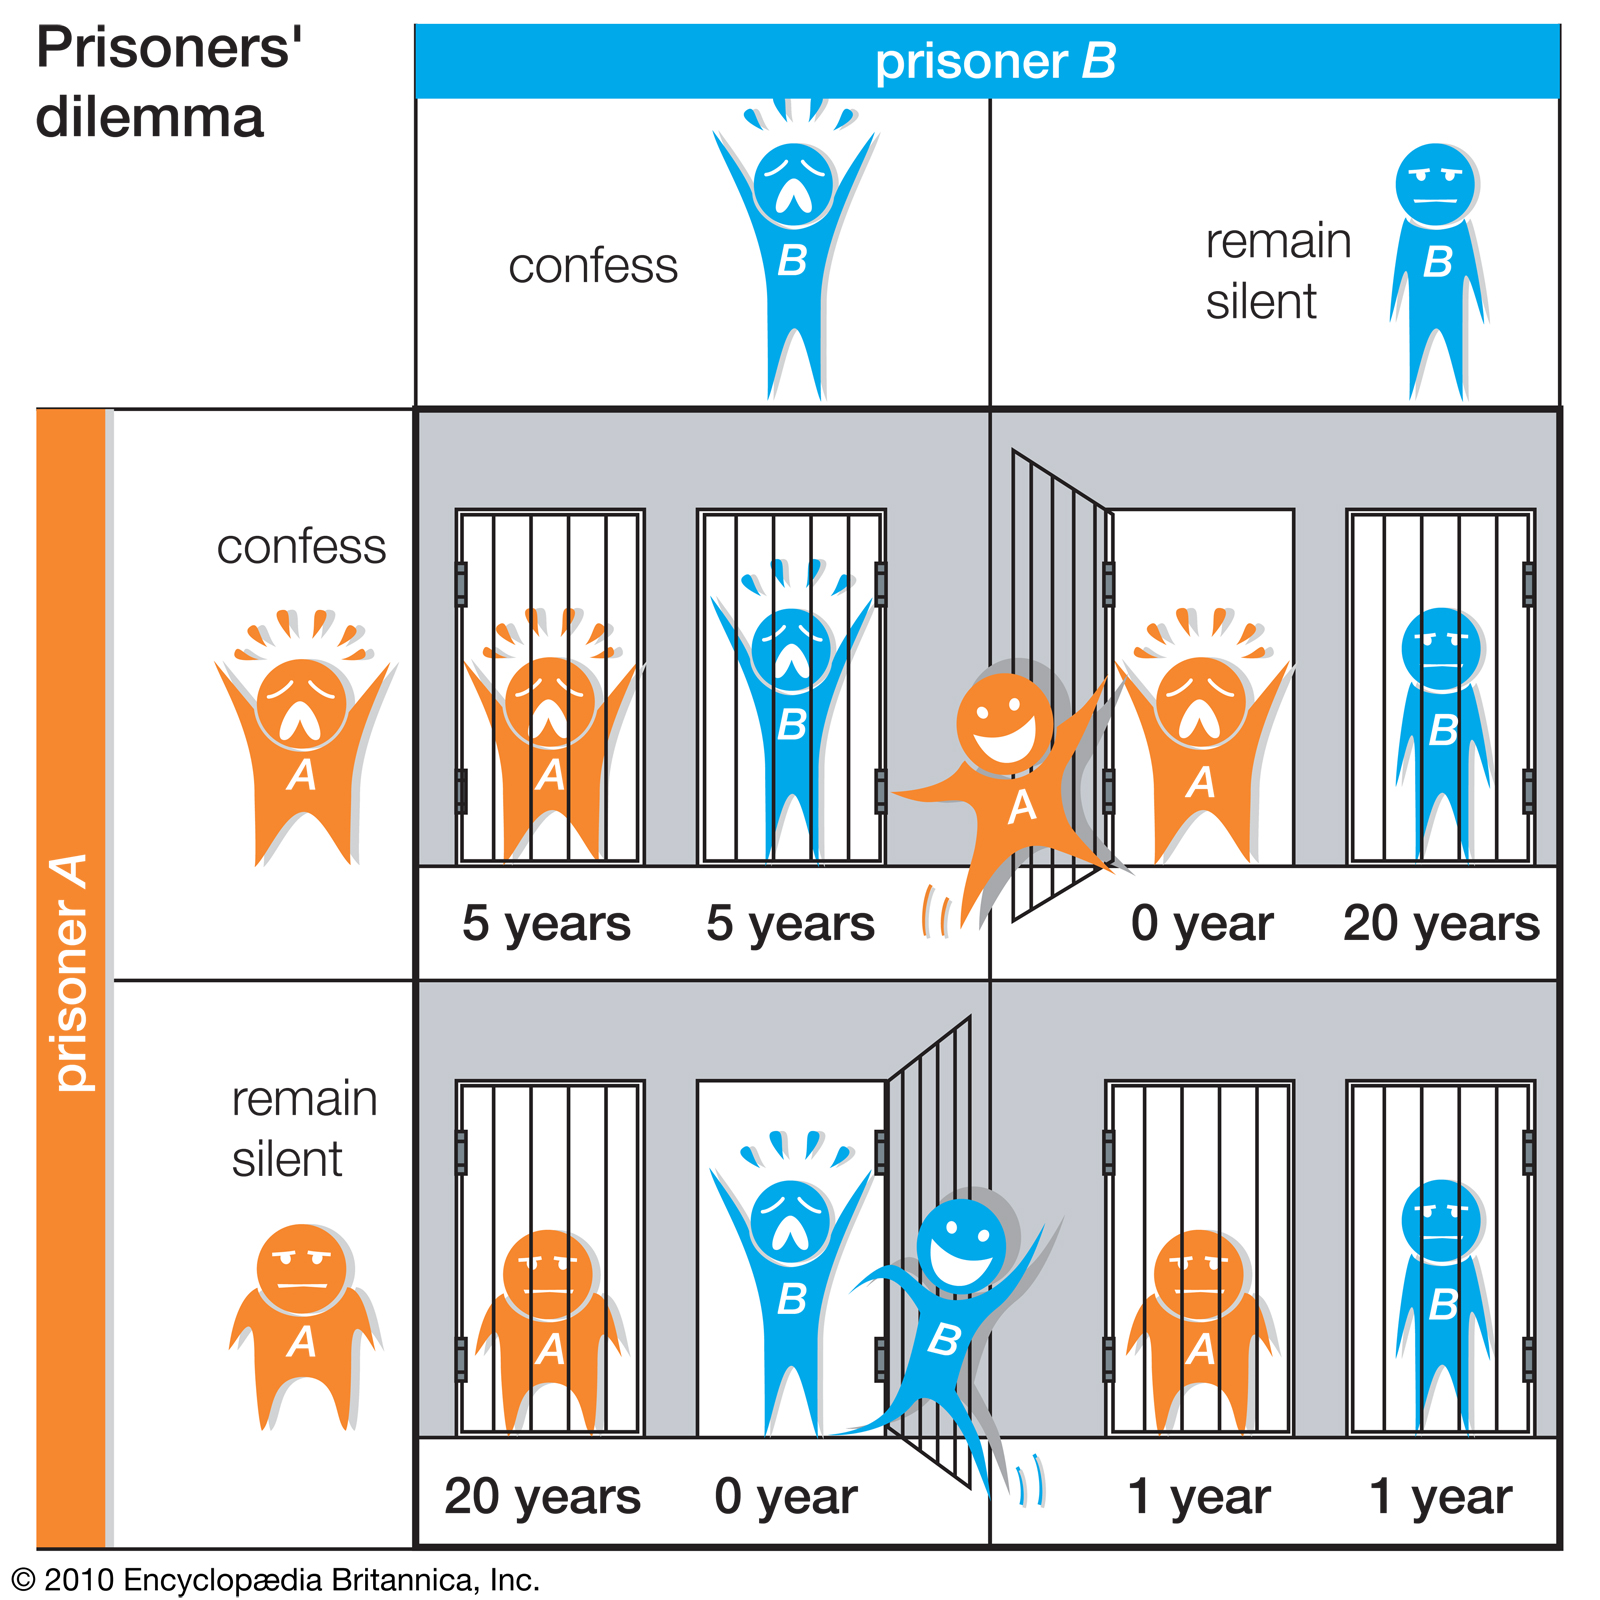
\includegraphics[width=.85\textheight, center]{prisoners_dilema}
}

%% Lets say for example that you have a 50% chance of surviving, And let us represent that chance by a fair toss of a coin that lands heads up. If you survive the fist toss - do you really want to toss the coin a second time? I hope it is perfectly obvious you do not as you have only a 25% chance of living through the second toss. Although the odds of any given toss are 50%,  you actually only have a 1 in 4 chance of heads coming up a second time in a row. Given that kind of math, a tails is almost certainly going to come along and ruin your day eventually. Try it for yourself. In my case, I got “No heads 48%” - so I would have died once out of every 2 duels. I think you will agree with me that you don’t want to have a gun fired at you hundreds if not thousands of times.

%
% SLIDE  ----------------------------------------------------------
%
\frame{\frametitle{Basic Statistics}
    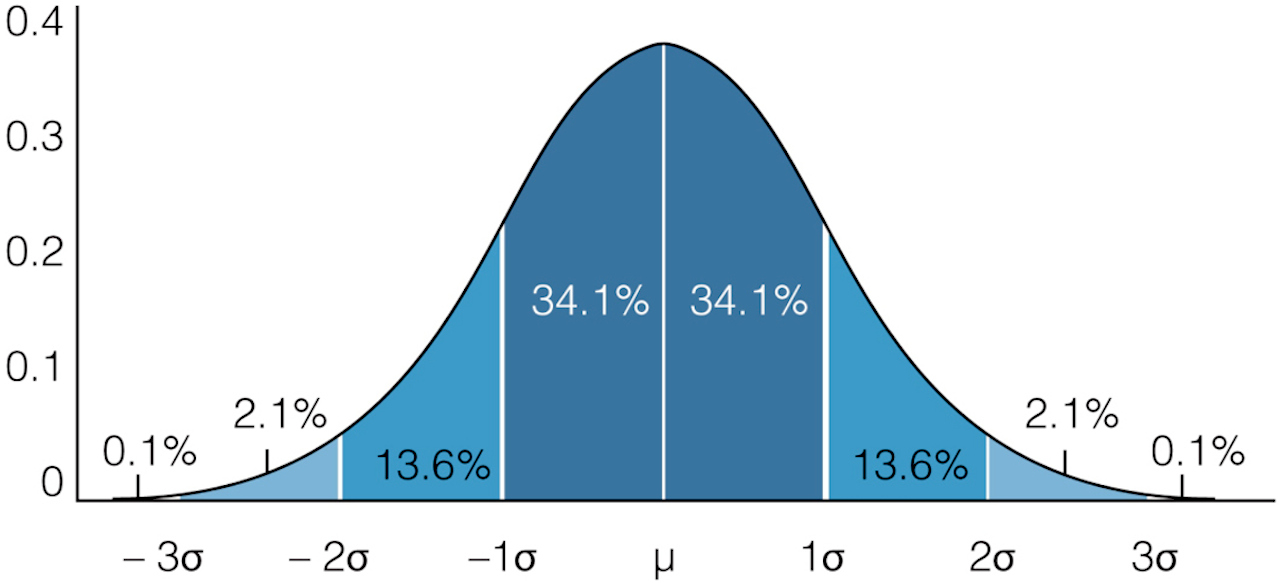
\includegraphics[width=.9\textwidth, center]{bell-curve}
}

%% We will assume that we are able to practice those 100 duel shots using blanks before noon tomorrow and learn the correct answer, perhaps we hired a consultant who could teach us the answer or a seasoned gunslinger who knows his trade. In the case of our web applications, this is not a penetration testing consultancy, but rather a subject matter expert in information security who is able to aid us with valuable strategic information that comes only from a lifetime of experiences in the field. We are now armed with knowledge about the ‘best strategy’ for survival in our duel tomorrow. 


%% To date I know that at least one of the security principles I have identified is a Pareto efficient one, and I believe that there are others. Incidentally, this principle happens to be one that most people have never heard of, and consequently never practice. This is the principle of Impact Reduction sometimes known as Risk Optimization. Although, it is rarely practiced, it is a very effective method. The goal of this principle is to examine ways that you can reduce the impact of events when the occur.

%
% SLIDE  ----------------------------------------------------------
%
\frame{\frametitle{Now For Something Completely Different}
    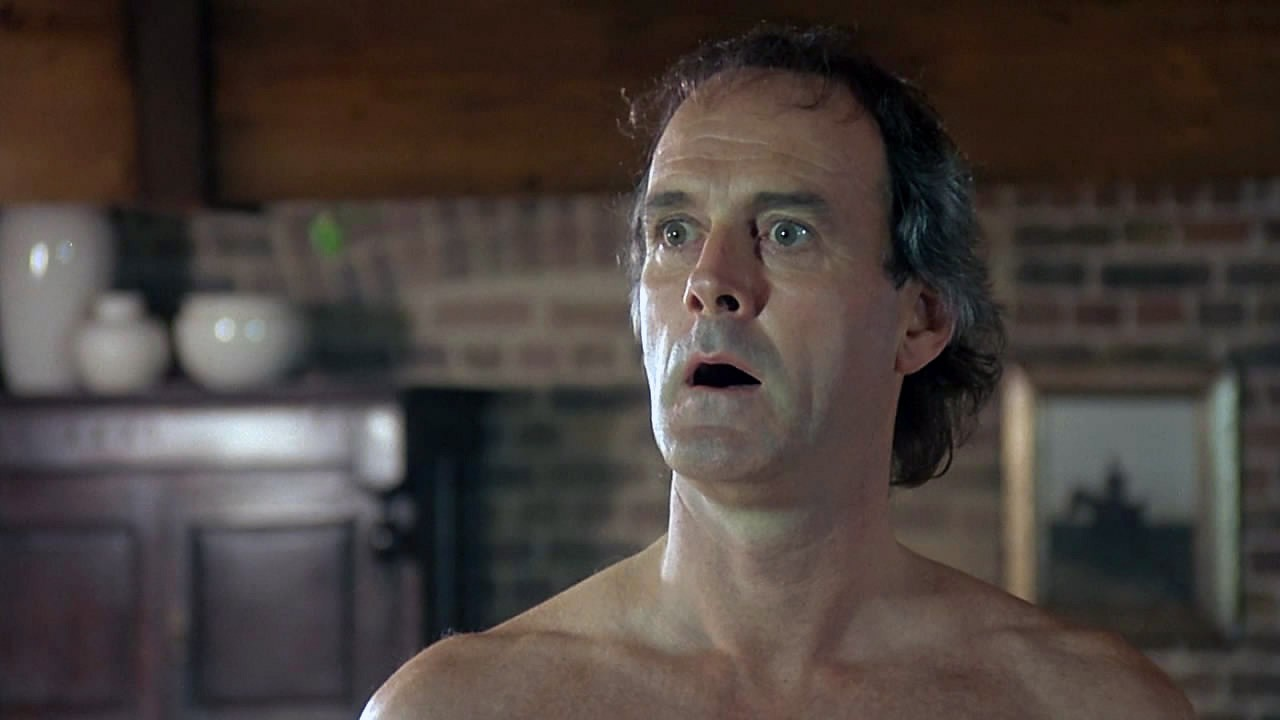
\includegraphics[width=.9\textwidth, center]{JohnCleese}
}

%
% SLIDE  ----------------------------------------------------------
%
\frame{\frametitle{Risk Optimization}
Risk Optimisation is rarely practiced, but highly effective method.
\begin{itemize}
	\item \alert {Reduce the impact of an event}
\end{itemize}
}

%% Returning to our pistol duel the most obvious way to implement the security principle of impact reduction is to wear a bullet proof vest! That is to say when we get hit by a bullet, it reduces the impact of the bullet when we get hit. Mind you, we still don’t want to get hit and are going to do our best to avoid it. And if we get hit, it is still going to hurt like crazy, but we will very likely survive. A bullet proof vest is obviously going to do more to save our lives at high noon tomorrow than all of the other 7 practices combined. 

%
% SLIDE  ----------------------------------------------------------
%
\frame{\frametitle{Bullet Proof Vest}
    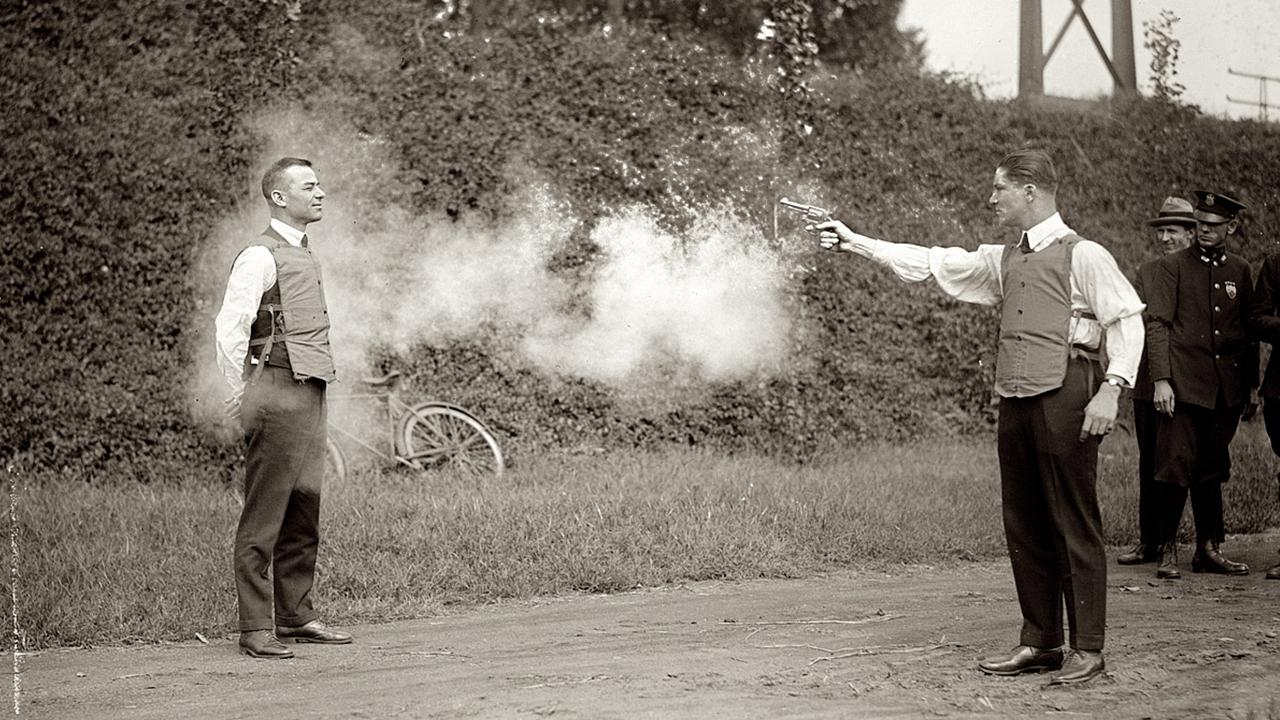
\includegraphics[width=.9\textwidth, center]{vest}
}

%% If we get hit our chances of survival are greatest if we have a bullet proof vest, but we would be equally foolish to rely on the bullet proof vest alone. Indeed we will still combine the bullet proof vest with the other 7 practices in order to maximize our chances of survival tomorrow. Naturally begs the question how do we apply an impact reduction strategy to our web applications? What do we do?

%
% SLIDE  ----------------------------------------------------------
% 

\frame{\frametitle{Security Principles}
\begin{itemize}
    \item{Know Yourself}
    \item{Use Time Based Security}
    \item{Know your Opponent}
    \item{Reduce Attack Surface}
    \item{Reluctance to Trust}
    \item{Add Impact Reduction}
    \item{Use Separation of Duty}
\end{itemize}
}


%
% SLIDE  ----------------------------------------------------------
%
\frame{\frametitle{How Can You Help?}
\begin{itemize}
	\item Join the Mailing List and Participate
	\item Help us develop reference implementations
	\item Tell your friends, and employers
\end{itemize}
}

%% We all know the devil is in the details, even bullet proof vests is not a one size fits all solution. Vests are rated according to the ability to stop different masses and speeds of projectiles. And the true is this is also true of OWASP AppSensor as well.

%% I sincerely hope that I have demonstrated sufficiently how important the philosophy and practice of impact reduction is, and why I am so excited about it. I hope that through this thought exercise that you will also be excited about it as well. Risk Optimization is actually how risk is managed across a wide range of disciplines outside of IT and it has been found to be very effective, and in my experience when applied to IT projects it has been equally effective.

%
% SLIDE  ----------------------------------------------------------
%
\frame{\frametitle{Obrigado!}
    
\includegraphics[width=.9\textwidth, center]{obrigado}
}


%
% SLIDE  ----------------------------------------------------------
%
\frame{\frametitle{Questions?}
    
\includegraphics[width=.9\textwidth, center]{Q_and_A}
}

%
% SLIDE  ----------------------------------------------------------
%
{\setbeamercolor{background canvas}{bg=o_blue}	
\begin{frame}[plain]
    
\includegraphics[width=.9\textheight, center]{owasp_logo_white}
\end{frame}
}

% ------------------------------------------------------------------------------
% End of Slides
% ------------------------------------------------------------------------------
\end{document}